\documentclass[12pt]{kiarticle}
\graphicspath{{pictures/}}
\DeclareGraphicsExtensions{.pdf,.png,.jpg,.eps}
%%%
\pagestyle{fancy}
\fancyhf{}
%\renewcommand{\headrulewidth}{ 0.1mm }
\renewcommand{\footrulewidth}{ .0em }
\fancyfoot[C]{\texttt{\textemdash~\thepage~\textemdash}}
\fancyhead[L]{Лабораторная работа № 6.11.5 \hfil}
\fancyhead[R]{\hfil Иванов Кирилл, 625 группа }
\usepackage{multirow} % Слияние строк в таблице
\newcommand
{\un}[1]
{\ensuremath{\text{#1}}}
\newcommand{\eds}{\ensuremath{ \mathscr{E}}}
\newcommand{\ga}{\ensuremath{\gamma}}
\usepackage{tikz}
%%% Работа с таблицами
\usepackage{array,tabularx,tabulary,booktabs} % Дополнительная работа с таблицами
\usepackage{longtable}  % Длинные таблицы
\usepackage{multirow} % Слияние строк в таблице

\begin{document}
	
	\begin{titlepage}
		\begin{center}
			\large 	Московский физико-технический институт \\
				(национальный исследовательский университет) \\
			Факультет общей и прикладной физики \\
			\vspace{0.2cm}
			
			\vspace{4.5cm}
			Лабораторная работа № 6.11.5 \\ \vspace{0.2cm}
			\large (Общая физика: квантовая физика) \\ \vspace{0.2cm}
			\LARGE \textbf{  Туннелирование в полупроводниках }
		\end{center}
		\vspace{2.3cm} \large
		
		\begin{center}
			Работу выполнил: \\
			Иванов Кирилл,
			625 группа
			\vspace{10mm}		
			
		\end{center}
		
		\begin{center} \vspace{60mm}
			г. Долгопрудный \\
			2019 год
		\end{center}
	\end{titlepage}


	\paragraph*{Цель работы:} исследовать принцип действия туннельного диода, измерить его вольт-амперную характеристику и основные параметры. 
	
	
	
	\section{Теоретическое введение}
	
	Туннельным диодом называется сильно легированный полупроводник, уровень Ферми которого лежит в разрешенной зоне и становятся возможны туннельные переходы электронов в области узкого $(p-n)$-перехода. 
	
	Будем считать, что все состояния, лежащие ниже уровня Ферми, заполнены электроны, а выше --- свободны. Энергетические диаграммы идеального туннельного диода и его вольт-амперная характеристика показаны на рисунке \ref{pic:diode}. $\mu_n$ и $\mu_p$ обозначены уровни Ферми в $n$- и $p$-области соответственно; $E_c$ и $E_v$ - границы зоны проводимости и валентной зоны. В отсутсвии внешнего поля уровни Ферми $\mu_n$ и $\mu_p$ лежат на одной горизонтали; число дырок и электронов, туннелирующих в обе стороны, одинаково, и ток отсутствует (рисунок \ref{pic:diode}.\textit{a}). При приложении напряжения в прямом направлении уровень Ферми в $n$-области <<ползет>> вверх по отношению к уровню Ферми в $p$-области, электроны туннелируют налево, ток растет. Он достигает максимума в точке \textit{б} вольт-амперной характеристики (рисунок \ref{pic:diode}.\textit{ж}), соответствующей наибольшему совпадению занятой зоны в отрицательной области и свободной в положительной. При дальнейшем увеличении внешнего напряжения перекрытие занятых уровней в $n$-области и свободных в $p$- уменьшается, и ток падает до нуля: это иллюстрирует рисунок \ref{pic:diode}.\textit{в}. Предельное положение соответствует энергетической диаграмме \textit{г}. При дальнейшем увеличении напряжения ток, возникающий за счет туннелирующих электронов, остается равным нулю, а диффузиозный ток возникает при совпадении занятых уровней $n$-области с свободными уровнями зоны проводимости (рисунок \ref{pic:diode}.\textit{д}). На диаграмме \ref{pic:diode}.\textit{е} показан ток в обратном направлении. 
	
	\begin{figure}[h]
		\centering	
		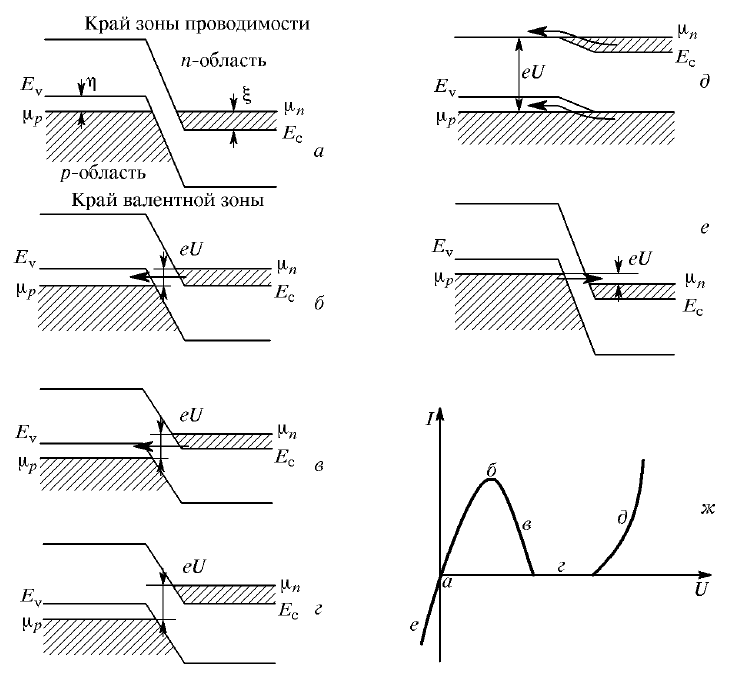
\includegraphics[width=0.5\textwidth]{diode.png}
		\caption{Схема энергетических уровней и вольт-амперная характеристика идеального туннельного диода}
		\label{pic:diode}
	\end{figure}  
	
	Реальная вольт-амперная характеристика туннельного диода отличается от таковой для идеального и представлена на рисунке \ref{pic:not_ideal}. Она учитывает образование примесных зон и возможность их слияния с основными, что объясняет наличия ненулевого тока $I_v$ в минимуме характеристики. 
	
	\begin{figure}[h]
		\centering	
		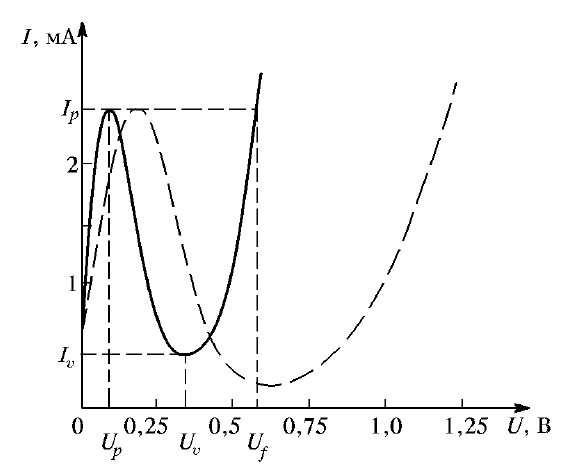
\includegraphics[width=0.4\textwidth]{not_ideal.png}
		\caption{Вольт-амперная характеристика неидеальных туннельных диодов с меньшей (сплошная линия) и большей (пунктирная линия) шириной запрещенной зоны}
		\label{pic:not_ideal}
	\end{figure}  
	
	Вольт-амперная характеристика реального туннельного диода (см. рисунок \ref{pic:not_ideal}) описывается следующими значениями напряжения и тока. 
	
	Напряжению $U_p$ соответствует максимум тока $I_p$, при котором смещение энергетических зон одинаково, причем это напряжение связано с расстоянием $\xi$ между уровнем Ферми в $n$-области и зоной проводимости и энергией $E_\text{n max}$, соответствующей максимуму плотности распределения электронов, следующим отношением: 
	
	\[ U_p \approx \frac{\xi - E_\text{n max}}{e} \]
	
	В точке $U_v$ ток минимален, и, как следует из описания выше:
	
	\[ U_v \approx \frac{(\mu_n - E_c) + (E_v - \mu_p)}{e} = \frac{\xi + \eta}{e} \approx \frac{2\xi}{e} \approx \frac{2\eta}{e} \]
	
	Напряжение $U_f$ характеризует раствор вольт-амперной характеристики и определяется шириной запрещенной зоны. 


	\section{Изучение вольт-амперной характеристики диода с помощью осциллографа}
	
	Схема установки представлена на рисунке \ref{pic:scheme_oscil}. На вход $ Y $ осциллографа подается напряжение, пропорциональное току через диод, а на вход $ X $ --- падение напряжения на диоде.
	
	\begin{figure}[h]
		\centering	
		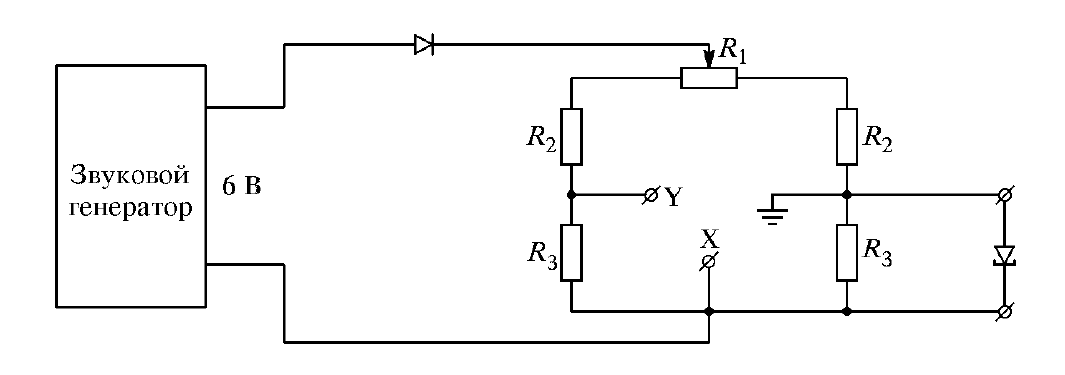
\includegraphics[width=0.5\textwidth]{scheme_oscil.png}
		\caption{Схема наблюдения вольт-амперной характеристики туннельного диода с помощью осциллографа}
		\label{pic:scheme_oscil}
	\end{figure}
	
	Ток $I$ через диод зависит от напряжения $U$ на нем по следующей формуле: 
	
	\[ I = U \frac{R_1 + 2(R_2 + R_3)}{(R_1 + 2R_2) \cdot R_3} \]
	
	Здесь $R_1$, $R_2$, $R_3$ --- сопротивления соответствующих резисторов моста со схемы на рисунке \ref{pic:scheme_oscil}. 
	
	Полученные осциллограммы для обычного и туннельного диода приведены на рисунках \ref{pic:ordinary_oscil} и \ref{pic:tunnel_oscil} соответственно. 
	
		\begin{figure}[h]
		\begin{minipage}[h]{0.49\linewidth}
		\centering	
		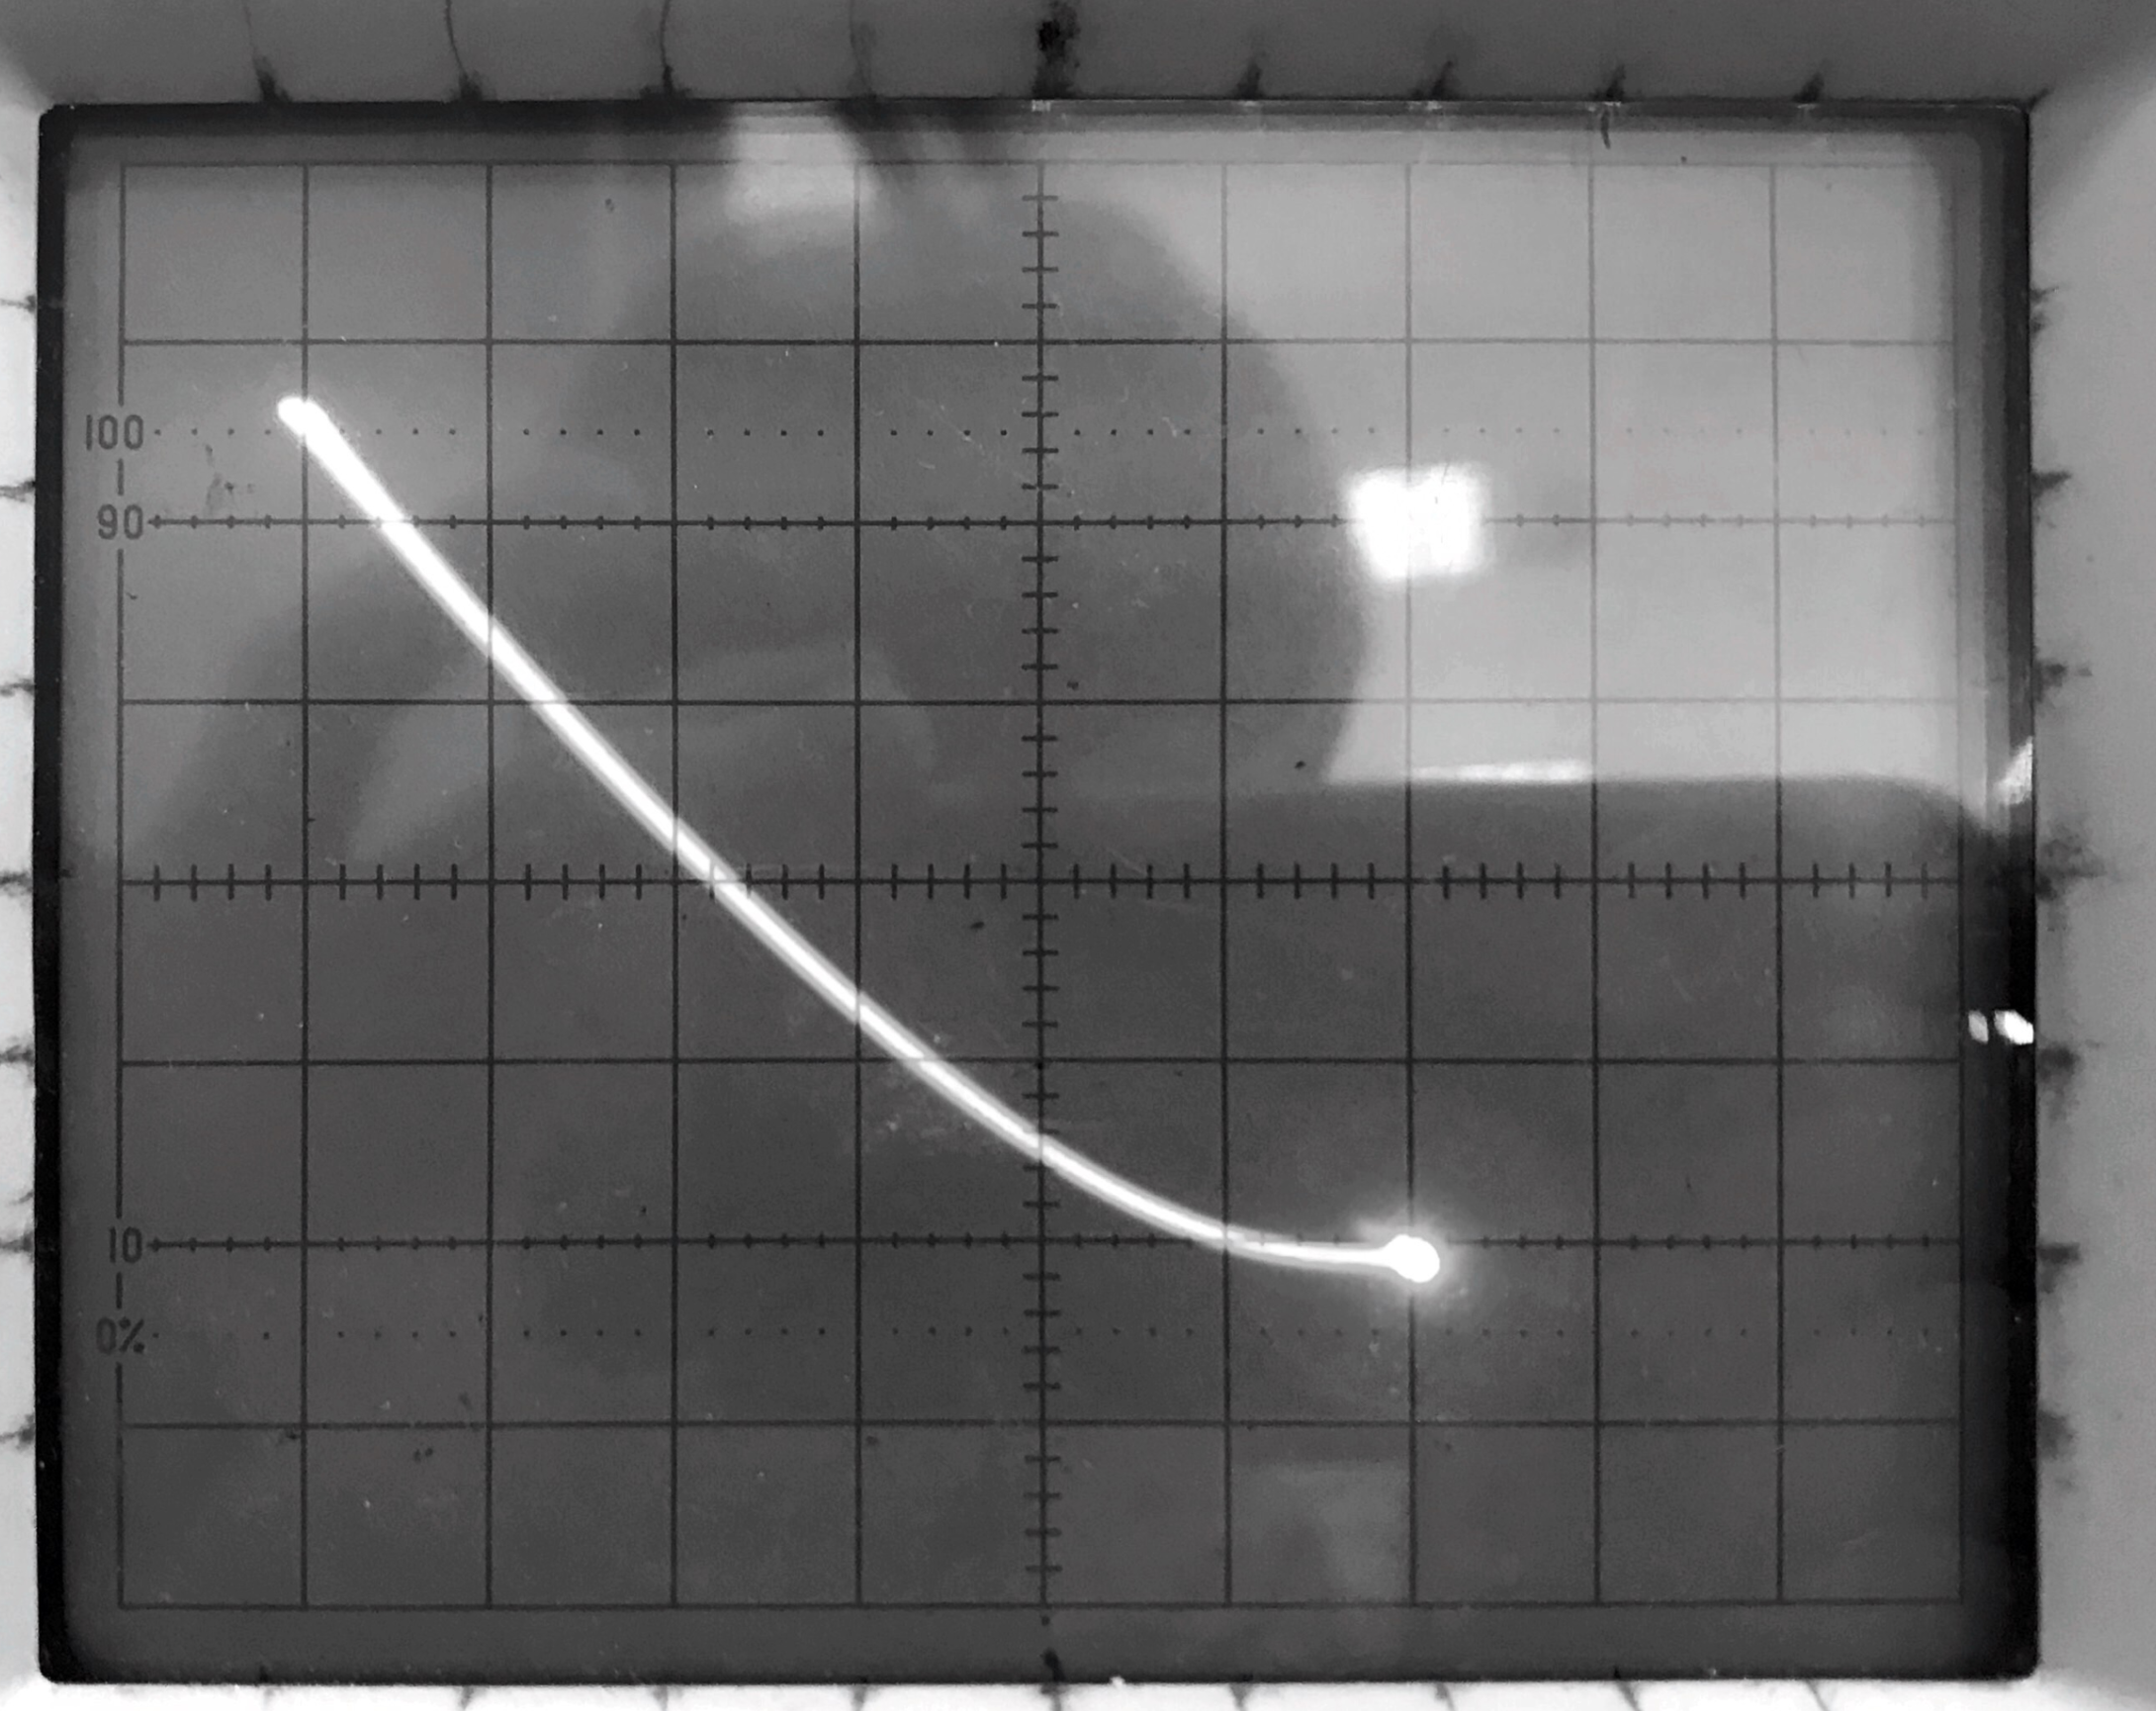
\includegraphics[width=0.9\textwidth]{o1.png}
		\caption{Вольт-амперная характеристика обычного полупроводникового диода на экране осциллографа}
		\label{pic:ordinary_oscil}
		\end{minipage}
		\begin{minipage}[h]{0.49\linewidth}
			\centering	
		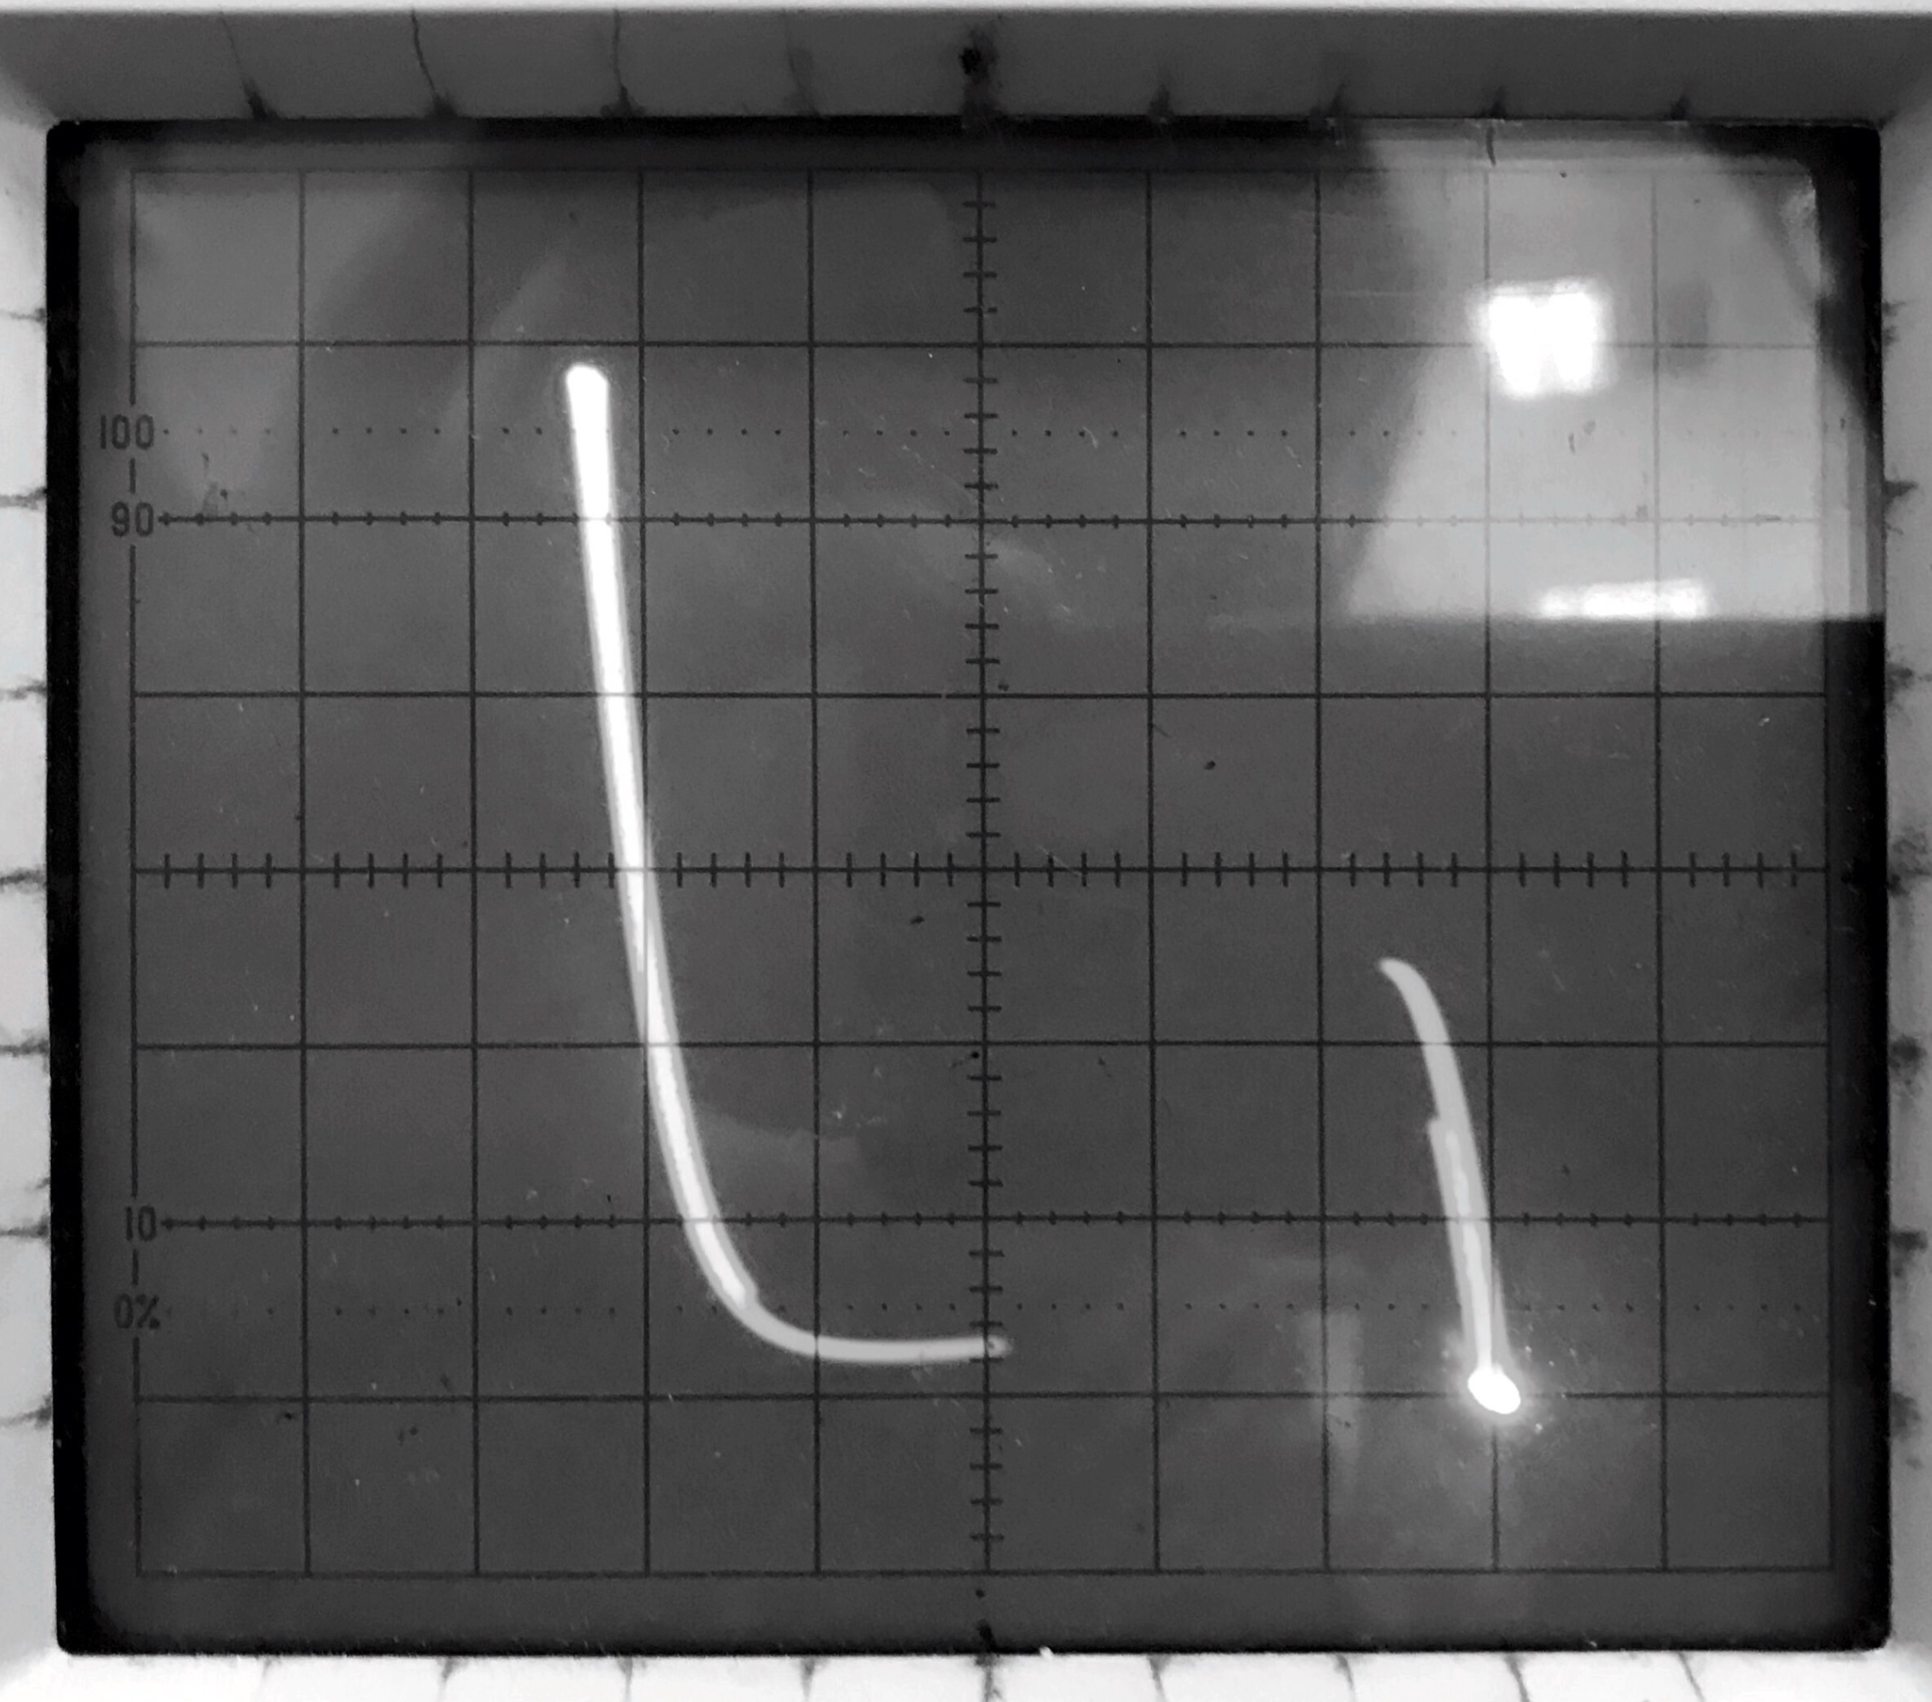
\includegraphics[width=0.82\textwidth]{o2.png}
		\caption{Вольт-амперная характеристика туннельного полупроводникового диода на экране осциллографа}
		\label{pic:tunnel_oscil}
		\end{minipage}
	\end{figure}
	
	
	
	По осциллограмме для туннельного диода (см. рисунок \ref{pic:tunnel_oscil}) оценим искомые величины напряжений (начало вольт-амперной характеристики соответствует нулевому напряжению): 
	
	\[ U_p \approx 0.07 \text{ В} \]
	\[ U_v \approx 0.4  \text{ В} \]
	\[ U_f \approx 0.5  \text{ В} \]
%	
%	Погрешность измерений примем равной половине цены маленького деления по оси.  
%	
%	С помощью формулы, указанной выше, вычислим токи в интересующих нас точках вольт-амперной характеристики: 
	
	
	\section{Получение статической характеристики туннельного диода}
	
		\begin{figure}[h]
		\centering	
		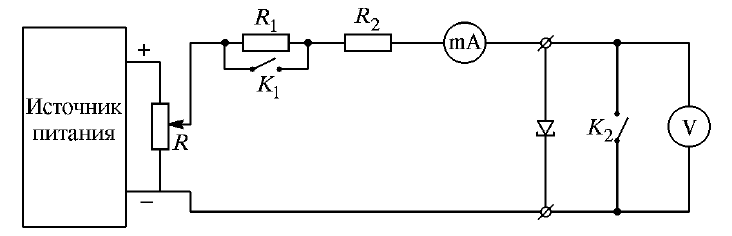
\includegraphics[width=0.5\textwidth]{scheme.png}
		\caption{Схема измерения параметров туннельного диода}
		\label{pic:scheme}
	\end{figure}
	
	Схема, используемая для получения статической характеристики диода, приведена на рисунке \ref{pic:scheme}. Ток измеряется миллиамперметром, включенным последовательно с диодом, а напряжение на диоде --- цифровым вольтметром. 
	
	Плавно меняя сопротивление резистора $ R $ и тем самым повышая напряжение на диоде, получим вольт-амперную характеристику туннельного диода $I(U)$.  Измерения приведены в таблице. Погрешность величин напряжения $U$ и тока $I$ оценим двумя единицами последнего разряда. По данным в таблице \ref{table_5} построим график зависимости $I(U)$. Он изображен на рисунке \ref{graf}. 
	
	\begin{figure}[h]
		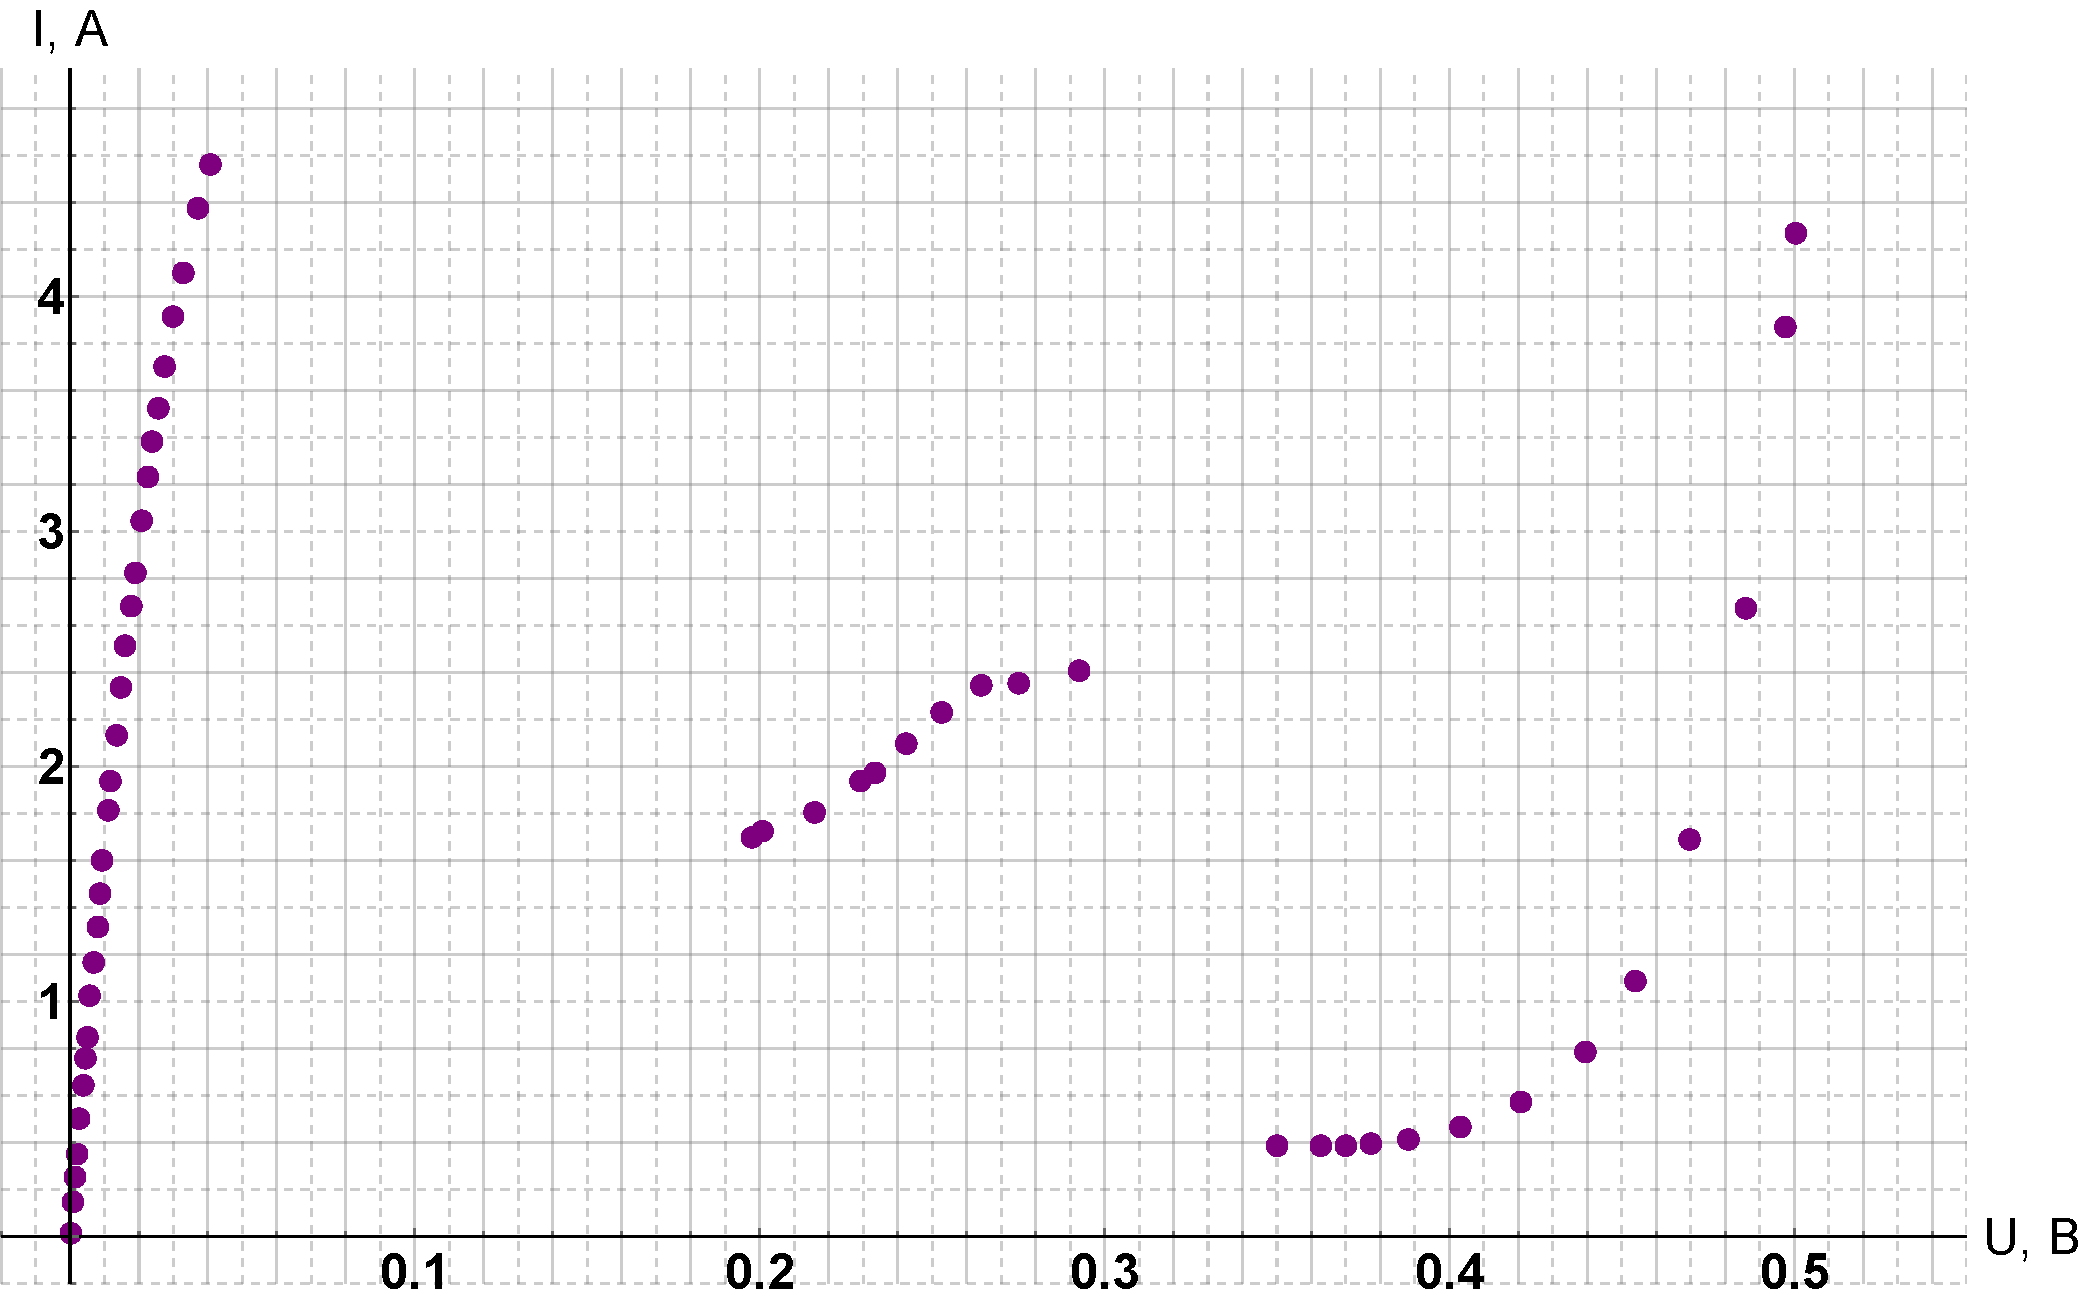
\includegraphics[scale=0.47]{graf.pdf}
		\caption{Измерение вольт-амперной характеристики $I(U)$ туннельного диода}
		\label{graf}
	\end{figure}
	
	\begin{table}[h]
		\caption{Результаты измерений}
		\begin{center}
			\begin{tabular}{|c|c|c|c|c|c|c|}
				\hline
				№ & $ U $, В & $ I $, А &  & № & $ U $, В & $ I $, А  \\
				\hline
			 1 & 0.0001 & 0.01 & \text{} & 27 & 0.0326 & 4.105 \\
			2 & 0.0009 & 0.145 & \text{} & 28 & 0.0371 & 4.378 \\
			3 & 0.0015 & 0.255 & \text{} & 29 & 0.0405 & 4.563 \\
			4 & 0.002 & 0.348 & \text{} & 30 & 0.1978 & 1.7 \\
			5 & 0.0029 & 0.504 & \text{} & 31 & 0.2011 & 1.724 \\
			6 & 0.0036 & 0.639 & \text{} & 32 & 0.2161 & 1.808 \\
			7 & 0.0043 & 0.761 & \text{} & 33 & 0.2295 & 1.934 \\
			8 & 0.0048 & 0.845 & \text{} & 34 & 0.2332 & 1.975 \\
			9 & 0.0059 & 1.028 & \text{} & 35 & 0.2425 & 2.095 \\
			10 & 0.0068 & 1.169 & \text{} & 36 & 0.2528 & 2.233 \\
			11 & 0.0078 & 1.32 & \text{} & 37 & 0.2645 & 2.347 \\
			12 & 0.0087 & 1.46 & \text{} & 38 & 0.2749 & 2.352 \\
			13 & 0.0096 & 1.604 & \text{} & 39 & 0.2928 & 2.405 \\
			14 & 0.011 & 1.817 & \text{} & 40 & 0.3498 & 0.385 \\
			15 & 0.0119 & 1.94 & \text{} & 41 & 0.3628 & 0.386 \\
			16 & 0.0133 & 2.135 & \text{} & 42 & 0.3698 & 0.39 \\
			17 & 0.0148 & 2.333 & \text{} & 43 & 0.377 & 0.397 \\
			18 & 0.0162 & 2.511 & \text{} & 44 & 0.3881 & 0.416 \\
			19 & 0.0175 & 2.68 & \text{} & 45 & 0.4034 & 0.464 \\
			20 & 0.0187 & 2.823 & \text{} & 46 & 0.421 & 0.57 \\
			21 & 0.0207 & 3.042 & \text{} & 47 & 0.4393 & 0.785 \\
			22 & 0.0225 & 3.231 & \text{} & 48 & 0.4537 & 1.091 \\
			23 & 0.024 & 3.384 & \text{} & 49 & 0.4699 & 1.692 \\
			24 & 0.0254 & 3.521 & \text{} & 50 & 0.4858 & 2.672 \\
			25 & 0.0274 & 3.703 & \text{} & 51 & 0.4974 & 3.871 \\
			26 & 0.03 & 3.912 & \text{} & 52 & 0.5005 & 4.267 \\
				\hline
			\end{tabular}
		\end{center}
		\label{table_5}
	\end{table}

	Из графика определим искомые значения токов и напряжений:
	
	\begin{itemize}
		\item $ U_p \approx 0,04 $ В, $ I_p' \approx 4,6 $ А
		\item $ U_v \approx 0,39 $ В, $ I_v \approx 0,4 $ А
		\item $ U_f \approx 0,51 $ В
	\end{itemize} 

Примем $E_v = 0$. Тогда из выражения для $U_v \approx 2\mu e$ можно найти энергию Ферми $\mu_n \approx \mu_p$:

\[ \mu_n \approx \mu_p \approx eU_v/2 \approx 0,195 \text{ эВ} \]

Из выражения для напряжения $U_p \approx (\mu_n - E_\text{n max})/e$ получим энергию, соответствующую максимальной плотности распределения электронов $E_\text{n max}$:

\[ E_\text{n max} = \mu_n - eU_p \approx 0,155 \text{ эВ} \] 
	
	\section{Вывод} 
	В работе исследован принцип действия туннельного диода; мы наблюдали его вольт-амперную характеристику на осциллографе и затем измерили ее непосредственно, снимая зависимость тока от напряжения. 
	
	По результатам измерений мы получили параметры диода, которые совпадают с грубой оценкой, полученной благодаря наблюдению на осциллографе.
	
\end{document}
